\documentclass{article}
\usepackage[margin=1in]{geometry}
\usepackage{mathtools, amsfonts, amsthm, graphicx, listings, xcolor, pdfpages}


\definecolor{codegreen}{rgb}{0,0.6,0}
\definecolor{codegray}{rgb}{0.5,0.5,0.5}
\definecolor{codepurple}{rgb}{0.58,0,0.82}
\definecolor{backcolour}{rgb}{0.95,0.95,0.92}

\lstdefinestyle{mystyle}{
    backgroundcolor=\color{backcolour},   
    commentstyle=\color{codegreen},
    keywordstyle=\color{magenta},
    numberstyle=\tiny\color{codegray},
    stringstyle=\color{codepurple},
    basicstyle=\ttfamily\footnotesize,
    breakatwhitespace=false,         
    breaklines=true,                 
    captionpos=b,                    
    keepspaces=true,                 
    numbers=left,                    
    numbersep=5pt,                  
    showspaces=false,                
    showstringspaces=false,
    showtabs=false,                  
    tabsize=2
}

\lstset{style=mystyle}

\title{HW05}
\author{Sam Ly}

\begin{document}
\maketitle

\section*{Required Exercise 1 [5]}
\begin{description}
    \item[Andy Zhang] {
        9/30/25, 11:36 AM

        ``
       Hi Andy, this is also for ex 1 hw05. I really liked your proof, it 
       was super slick and a lot more straight forward than what I came up with. 
       I really like how you explicitly state how you are substituting the equations.
        But that is also where I would have some constructive criticism. The proof 
        itself is fine, but a latex tip is to use the reference command in order to refer back to previous work in a semantically correct way. Otherwise, I thought it was a great proof! Another thing is that the long string of display style math could have been better suited with a inline math. That way, the sentences flow better visually. Lastly, the wording of the conclusion of the proof seems a bit odd to me. Maybe something like "Therefore, we see that <expression> must be divisible by m, and that <expression> is congruent to <expression>." 
        ''
    }

    \item[Sox] {
        9/30/25, 9:56 PM

        ``
        Hi Sox, this is for HW5 ex 1.

I really liked your proof, and thought it was intuitive and easy to follow. Here are the four pieces of feedback:
1. The structure of proof made a lot of sense. Proving the smaller statements before combining them in the final conclusion sentence made a lot of sense.
2. I like how you included multiple base cases to make the proof more concrete.
3. Some of the math isn’t in “complete sentences.” For example, The middle block of display style math doesn’t end with a period. This is nitpicky, but I didn’t really see anything else.
4. Overall, I thought this was a really good proof, but there were just some little formatting things like the “4m” at the start of the proof not being inline math.
        ''
    }
\end{description}


\section*{Required Exercise 2 [3]}

\begin{enumerate}
    \item {
        Prove that for all integers \(n \ge 2\), 
        \[\left( A_1 \cup A_2 \cup ... \cup A_n \right)^c = A_1^c \cap A_2^c \cap ... \cap A_n^c \]

        \begin{proof}
            First, we define some useful notation for a union and intersection
            for a large series of sets \(A_1, A_2, ..., A_3\):
            \[ \bigcup_{i=1}^{n} A_i = A_1 \cup A_2 \cup ... \cup A_n\]
            \[ \bigcap_{i=1}^{n} A_i = A_1 \cap A_2 \cap ... \cap A_n.\]

            First, we use the standard De Morgan's Law as the base case \(n=2\),
            \(\left( A_1 \cup A_2 \right)^c = A_1^c \cap A_2^c.\)

            Then, as our inductive hypothesis, we assume that 
            \[ \left( \bigcup_{i=1}^{n} A_i \right)^c = \bigcap_{i=1}^{n} A_i^c, \text{ for } n \le k.\]

            Then, we see that for \(n+1\), 
            \begin{align*}
                \left( \bigcup_{i=1}^{n+1} A_i \right)^c &= \left( \bigcup_{i=1}^{n} A_i \cup A_{n+1} \right)^c \\
                \left( \bigcup_{i=1}^{n+1} A_i \right)^c &= \left( \bigcup_{i=1}^{n} A_i \right)^c \cap A_{n+1}^c .\\
            \end{align*}

            We can use our inductive hypothesis to substitute 
            \(\left( \bigcup_{i=1}^{n} A_i \right)^c = \bigcap_{i=1}^{n} A_i^c\)
            to get,
            \begin{align*}
                \left( \bigcup_{i=1}^{n+1} A_i \right)^c &= \bigcap_{i=1}^{n} A_i^c \cap A_{n+1}^c .\\
                &= A_1^c \cap A_2^c \cap ... \cap A_n^c \cap A_{n+1}^c .\\
            \end{align*}

            Therefore, 
            \[\left( A_1 \cup A_2 \cup ... \cup A_n \right)^c = A_1^c \cap A_2^c \cap ... \cap A_n^c \]
            for any integer \(n \ge 2\).
        \end{proof}
    }

    \item {
        Prove that for all integers \(n \ge 2\), 
        \[\left( A_1 \cap A_2 \cap ... \cap A_n \right)^c = A_1^c \cup A_2^c \cup ... \cup A_n^c \]

        \begin{proof}
            First, we use the standard De Morgan's Law as the base case \(n=2\),
            \(\left( A_1 \cap A_2 \right)^c = A_1^c \cup A_2^c.\)

            Then, as our inductive hypothesis, we assume that 
            \[ \left( \bigcap_{i=1}^{n} A_i \right)^c = \bigcup_{i=1}^{n} A_i^c, \text{ for } n \le k.\]

            Then, we see that for \(n+1\), 
            \begin{align*}
                \left( \bigcap_{i=1}^{n+1} A_i \right)^c &= \left( \bigcap_{i=1}^{n} A_i \cap A_{n+1} \right)^c \\
                \left( \bigcap_{i=1}^{n+1} A_i \right)^c &= \left( \bigcap_{i=1}^{n} A_i \right)^c \cup A_{n+1}^c .\\
            \end{align*}

            We can use our inductive hypothesis to substitute 
            \(\left( \bigcap_{i=1}^{n} A_i \right)^c = \bigcup_{i=1}^{n} A_i^c\)
            to get,
            \begin{align*}
                \left( \bigcap_{i=1}^{n+1} A_i \right)^c &= \bigcup_{i=1}^{n} A_i^c \cup A_{n+1}^c .\\
                &= A_1^c \cup A_2^c \cup ... \cup A_n^c \cup A_{n+1}^c .\\
            \end{align*}

            Therefore, 
            \[\left( A_1 \cap A_2 \cap ... \cap A_n \right)^c = A_1^c \cup A_2^c \cup ... \cup A_n^c \]
            for any integer \(n \ge 2\).
        \end{proof}
    }
\end{enumerate}

\section*{Required Exercise 3 [2]}
See below.

\section*{Choice Exercise 6 [5]}

\begin{enumerate}
    \item {
        \begin{description}
            \item[My original guess:] {
                We say 
                \[p(x) \equiv q(x) \pmod{r(x)}\]
                if there exists an integer \(k\) such that \(p(x) - q(x) = k \times r(x)\).
            }
            \item[Comparison:] {
                My original guess was wrong because the actual definition for 
                this relation is that there exists a function \(f(x)\) such that 
                \(p(x) - q(x) = f(x) \times r(x)\).

                My original guess is actually a special case of the actual definition,
                since \(f\) can be a constant function. However, my original guess 
                is also wrong in a more subtle way because the actual definition of 
                polynomial congruence extends to the real numbers, while my 
                original guess only relates to the natural numbers.
            }
        \end{description}
    }

    \item {
        [1] Recall that if we're given two (positive) integers n=\(n\) and \(m\)
        and their decimal representation, it's easy to check \(n  \equiv m \pmod{10}\):
        just make sure that their last digits match up. What is the analgous rule 
        when looking at polynomials \(\mod{x}\)?

        First, we notice that decimal is a positional number system, and \(10\)
        is one of bases. This makes it easy to check for congruence under \(\mod{10}\)
        because for integer \(n\), if the one's place of number is 0, then 
        \(n \equiv 0 \pmod{10}\). Analogously, polynomials can themselves be see 
        as a "positional number system" where each degree term is a position. Thus, 
        any time a polynomial \(p(x)\) has no constant term (analogous to the one's place), 
        \(p(x) \equiv 0 \pmod{x}\). We see this intuitively when we write out 
        examples of \(p(x)\). For example,
        \[p(x) = x^2 + 3x = x(x + 3).\]
    }

    \item {
        [1] Prove that \(x^2 \equiv -1 \pmod{x^2 + 1}\).

        We see that \(p(x) = x^2\) and \(q(x) = -1\), thus 
        \[x^2 - (-1) = (x^2 + 1) \times f(x),\]
        for some \(f\). 

        We see that \(f(x) = 1\). Thus, \(x^2 \equiv -1 \pmod{x^2 + 1}\).
    }

    \item {
        [1] Notice that you can replace every \(x^2\) with \(-1\) when simplifying 
        a polynomial \(\mod{x^2 + 1}\). Use this to simplify \(x^4 + x^2 + 1 \pmod{x^2 + 1}\).

    }
\end{enumerate}

\section*{Choice Exercise 7 [3]}

\begin{enumerate}
    \item {
        Choose a programming language, determine the logical operators, write a truth table, and record the results here.

        \lstinputlisting[language=Python, lastline=12]{./code/main.py}
    }

    \item {
        We can have a truth table which has three columns recording values, 
        \(P\), \(Q\), and \(R\). This means that there are \(2^{2^3} = 256\) 
        different logical statements we can make up to logical equivalence. 
        Write a program that outputs a logical statement for each different outcome.

        \lstinputlisting[language=Python, firstline=14]{./code/main.py}
    }
\end{enumerate}

\section*{Choice Exercise 8 [3]}
\emph{I will use the \(\neg\) for negation because the bot uses this notation.}
\begin{enumerate}
    \item {
        \(((a \Leftrightarrow b) \vee \neg (\neg a \Leftrightarrow a))\)

        First, we notice that \(\neg a \Leftrightarrow a\) is always false. Thus, 
        \(\neg (\neg a \Leftrightarrow a))\) is always true. Therefore, the entire 
        statement is always true.
    }

    \item {
        \((a \Leftrightarrow b) \vee \neg \neg (b \vee a)\)

        First, we see that the double negation can be simplified to yield
        \((a \Leftrightarrow b) \vee (b \vee a)\).
        Then, we see that there are two possible cases:
        \begin{description}
            \item[\(a \not\Leftrightarrow b\)] {
                When this is the case, then \(b \vee a \) must be true since 
                one of the variables must be true.
            }
            \item[\(a \Leftrightarrow b\)] {
                When both variables are false or true, this statement is true. 
            }
        \end{description}

        Thus, there is no combination of \(a\) and \(b\) that makes the statement false.
    }

    \item {
        \((a \Leftrightarrow a) \rightarrow (\neg a \Leftrightarrow \neg a)\).

        First, we notice that \(\neg \Leftrightarrow \neg a \) is always true. 
        This means that the overall implication is also alaways true.
    }
\end{enumerate}


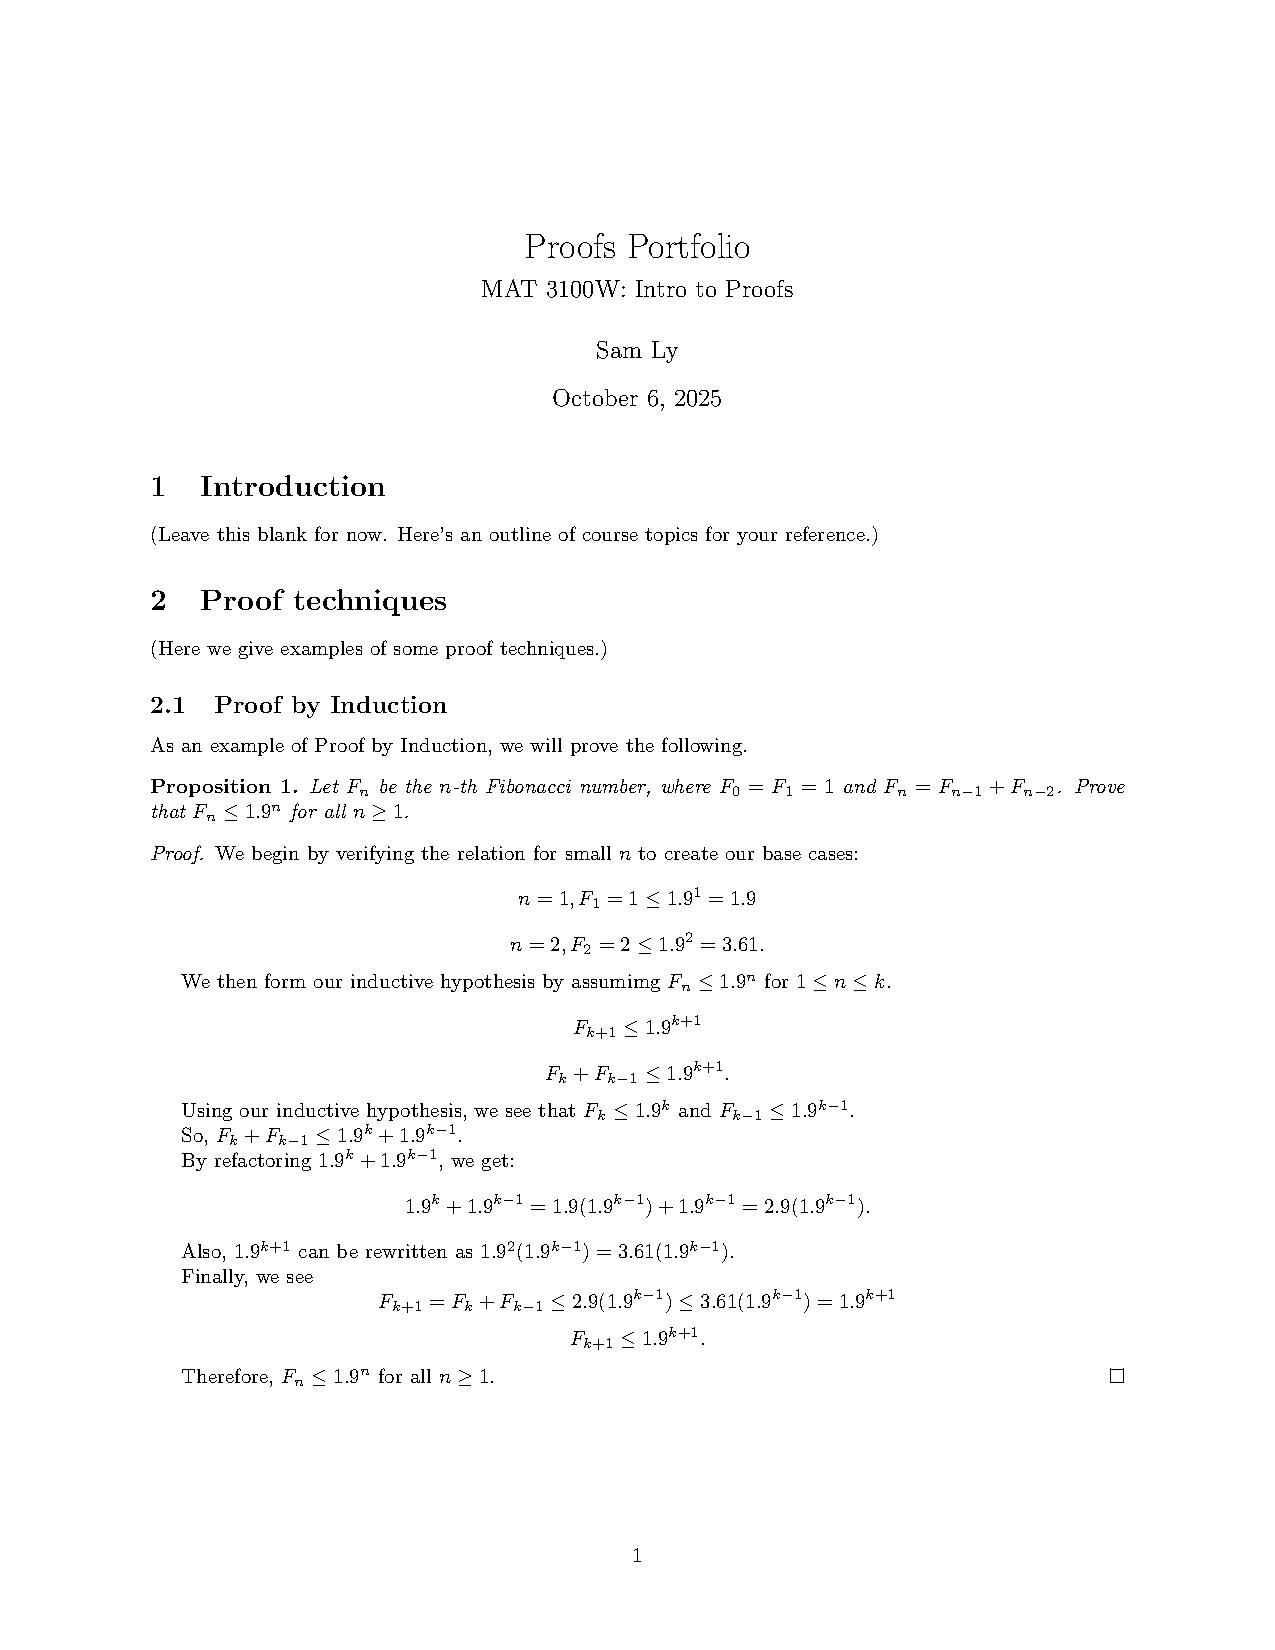
\includepdf[pages=-]{portfolio.pdf}
\end{document}